\documentclass[12pt,a4paper]{article}
\usepackage[utf8]{inputenc}
\usepackage[utf8]{vietnam}
\usepackage{amsmath,amsfonts,amssymb}
\usepackage{xfrac}
\usepackage{type1cm}
\usepackage{graphicx}
\usepackage{subfig}
\graphicspath{ {images/} }
\usepackage{multirow}
\usepackage{multicol}
\usepackage{array}
\usepackage{comment}
\usepackage{enumerate}
\usepackage[unicode, hidelinks = true]{hyperref}
\usepackage{indentfirst}
\usepackage{tikz}
\usepackage{color}
\usepackage[left=2cm,right=2cm,top=2cm,bottom=2cm]{geometry}
\usepackage[american,cuteinductors,smartlabels]{circuitikz}
\usetikzlibrary{arrows}
\usepackage{tikz}
\usetikzlibrary{calc,patterns,angles,quotes}
\usetikzlibrary{arrows, decorations.markings, calc, fadings, decorations.pathreplacing, patterns, decorations.pathmorphing, positioning}	
%\tikzstyle{every path}=[line width=1.2pt]
\title{\textbf{BÁO CÁO KIỂM TRA GIỮA KỲ \vspace{1cm} \\ CHỦ ĐỀ BÁO CÁO \vspace{.3cm} \\ ỨNG DỤNG KỸ THUẬT LẬP TRÌNH TUẦN TỰ TRONG THIẾT KẾ HỆ THỐNG ĐIỀU KHIỂN\vspace{0.5cm}}\\Môn học: Thiết kế hệ thống điều khiển\vspace{.4cm}\\Lớp: Công nghệ, kỹ thuật điện, điện tử}
\author{GVHD: Nguyễn Khắc Nguyên \and Nhóm SVTH: Nhóm 4}
\date{Thời gian: Ngày 08 tháng 11 năm 2016}
%Ứng dụng kỹ thuật lập trình tuần tự trong thiết kế hệ thống điều khiển
\tikzset{middlearrow/.style={
        decoration={markings,
            mark= at position 0.5 with {\arrow{#1}} ,
        },
        postaction={decorate}
    }
}

\begin{document}
\pagenumbering{gobble}
\maketitle
\everymath{\displaystyle}
%%
%%
%\tableofcontents
%\listoffigures
%\listoftables
%\newpage
\pagenumbering{arabic}
\renewcommand{\arraystretch}{1.3}

\section*{Danh sách sinh viên nhóm 4}
		\begin{tabular}{cp{3.5cm}c}%\hline
			%\textbf{STT} & \centering{\textbf{Họ và tên SV}} & \textbf{MSSV} \\ \hline
			1. & Nguyễn Văn Đình & MSSV: 1350353 \\ %\hline
			2. & Thi Minh Nhựt & MSSV: 1350366 \\ %\hline
			3. & Phạm Thanh Quý & MSSV: 1350222 \\ %\hline
			4. & Hồ Minh Thành & MSSV: 1350444 \\ %\hline
			5. & Liên Thái Trường & MSSV: 1350358 \\ %\hline
			6. & Lư Anh Tuấn & MSSV: 1350240 \\ %\hline
		\end{tabular}
\section{Chủ đề báo cáo}
%\subsection*{Đề bài -- Bài tập 4 -- Nhóm 4}
\subparagraph{Đề bài -- Bài tập 4 -- Nhóm 4} Cho quá trình có sơ đồ như hình \ref{Fig:debai-baocao}:
	%Cho quá trình có sơ đồ như hình \ref{Fig:debai-baocao}:
		\begin{figure}[!h]
			\begin{center}
				\begin{tikzpicture}[>=triangle 45]
					\draw (5,0) node {\small{$Start~A+D+D-G+G-A-A+B+A-B-\left\{\begin{array}{c}D+E+E-D-\\ \\G+G-H+H-\end{array}\right\}E+B+B-H+E-H-$}};
					\draw (1.9,-0.2) -- (1.9,-1) -- (-2.7,-1); \draw (-0.4,-1) node[above]{$2 \textrm{ lần }$};
						
					\draw (13.8,-0.2) -- (13.8,-2) -- (-2.7,-2); \draw[->](-2.7,-2) -- (-2.7,-0.2); \draw (12.55,-2) node[above]{$\overline{Stop}$};
				\end{tikzpicture}
			\end{center}
			\caption{Sơ đồ quá trình của bài tập 4 - nhóm 4} \label{Fig:debai-baocao}
		\end{figure}

%\subsection*{Yêu cầu}
\subparagraph{Yêu cầu}
	\begin{enumerate}
		\item Viết \emph{sơ đồ logic} và \emph{sơ đồ cấp điện} cho quá trình trên \emph{hình \ref{Fig:debai-baocao}}. \label{ex:sodologic}
	
		
		\item Sử dụng \emph{phần mềm Festo Fluidsim} \emph{mô phỏng quá trình} cho trên \emph{hình \ref{Fig:debai-baocao}} để kiểm chứng lại kết quả trong câu \ref{ex:sodologic}. Mô phỏng theo các cách sau:
			\begin{enumerate}
				\item Xây dựng \emph{sơ đồ nối điện.}
				
				\item Xây dựng sơ đồ Leader.
				
				\item Sử dụng \emph{ngôn ngữ lập trình PLC}, thực hiện \emph{kết nối PLC SIM và Festo Fluidsim} để mô phỏng quá trình.
			\end{enumerate}
	\end{enumerate}
	
\section{Nội dung báo cáo}
%\subsection*{Bài tập 4 -- Nhóm 4}
\subparagraph{Đề bài -- Bài tập 4 -- Nhóm 4} Cho sơ đồ quá trình như hình \ref{Fig:quatrinh-tuantu-baitap4}:
			\begin{figure}[!h]
				\begin{center}
					\begin{tikzpicture}[>=triangle 45]
						\draw (5,0) node {\small{$Start~A+D+D-G+G-A-A+B+A-B-\left\{\begin{array}{c}D+E+E-D-\\ \\G+G-H+H-\end{array}\right\}E+B+B-H+E-H-$}};
						\draw (1.9,-0.2) -- (1.9,-1) -- (-2.7,-1); \draw (-0.4,-1) node[above]{$2 \textrm{ lần }$};
						
						\draw (13.8,-0.2) -- (13.8,-2) -- (-2.7,-2); \draw[->](-2.7,-2) -- (-2.7,-0.2); \draw (12.55,-2) node[above]{$\overline{Stop}$};
					\end{tikzpicture}
				\end{center}
				\caption{Sơ đồ quá trình bài tập 4 -- nhóm 4}\label{Fig:quatrinh-tuantu-baitap4}
			\end{figure}
			
			\begin{itemize}
				\item \emph{Bước 1 -- Bước 2: Gom nhóm và đặt tên cho các nhóm}.
				
				Thực hiện chia nhóm và đặt tên cho các nhóm được sơ đồ như hình \ref{Fig:quatrinh-tuantu-baitap4-gomnhom}.
					\begin{figure}[!h]
						\begin{center}
							\begin{tikzpicture}[>=triangle 45]
								\draw (5,0) node {\small{$Start~A+D+D-G+G-A-A+B+A-B-\left\{\begin{array}{c}D+E+E-D-\\ \\G+G-H+H-\end{array}\right\}E+B+B-H+E-H-$}};
								\draw (1.9,-0.3) -- (1.9,-1) -- (-2.7,-1); \draw (0,-1) node[above]{$2 \textrm{ lần }$}; \draw (1.9,-0.5) node[right]{$cnt=1$}; \draw (-1.8,-1) node[above]{$cnt=0$};
						
								\draw (13.8,-0.3) -- (13.8,-2) -- (-2.7,-2); \draw[->](-2.7,-2) -- (-2.7,-0.3); \draw (12.55,-2) node[above]{$\overline{Stop}$}; \draw (-2.2,-2) node[above]{$ys$};
								\draw[thick] (-2.6,0.5) -- (-2.8,-0.2);
								\draw[thick] (-1,0.5) -- (-1.2,-0.2); \draw (-1.75,0.5) node[above]{$y_1$};
						
								\draw[thick] (0.55,0.5) -- (0.35,-0.2); \draw (-0.25,0.5) node[above]{$y_2$};
						
								\draw[thick] (2.1,0.5) -- (1.9,-0.2); \draw (1.25,0.5) node[above]{$y_3$};
						
								\draw[thick] (3.65,0.5) -- (3.45,-0.2); \draw (2.875,0.5) node[above]{$y_4$};
						
								\draw[thick] (5.15,0.5) -- (5,-0.2); \draw (4.4,0.5) node[above]{$y_5$};
						
								\draw[thick] (5.6,1) -- (5.5,0.3);
								\draw[thick] (7.2,1) -- (7.1,0.3); \draw (6.175,1) node[above]{$y_6$};
						
								\draw[thick] (8.7,1) -- (8.6,0.3); \draw (7.95,1) node[above]{$y_7$};
							
								\draw[thick] (5.6,0) -- (5.45,-.8);
								\draw[thick] (6.4,0) -- (6.25,-.8); \draw (5.8,-.8) node[below]{$y_8$};
						
								\draw[thick] (7.2,0) -- (7.05,-.8); \draw (6.7,-0.8) node[below]{$y_9$};
						
								\draw[thick] (8,0) -- (7.85,-.8); \draw (7.5,-.8) node[below]{$y_{10}$};
						
								\draw[thick] (8.8,0) -- (8.65,-.8); \draw (8.3,-.8) node[below]{$y_{11}$};
						
								\draw[thick] (9.2,0.5) -- (9.05,-0.2);						
								\draw[thick] (10.8,0.5) -- (10.65,-0.2); \draw (10,.5) node[above]{$y_{12}$};
						
								\draw[thick] (12.4,0.5) -- (12.25,-0.2); \draw (11.6,.5) node[above]{$y_{13}$};
						
								\draw[thick] (14,0.5) -- (13.85,-0.2); \draw (13.2,.5) node[above]{$y_{14}$};
							\end{tikzpicture}
						\end{center}
						\caption{Sơ đồ quá trình sau khi đã gom nhóm và đặt tên cho các nhóm} \label{Fig:quatrinh-tuantu-baitap4-gomnhom}
					\end{figure}
				
				\item \emph{Bước 3: Viết sơ đồ logic cho quá trình.}
					
					\begin{figure}[!h]
						\vspace{-.8cm}
						\begin{center}
							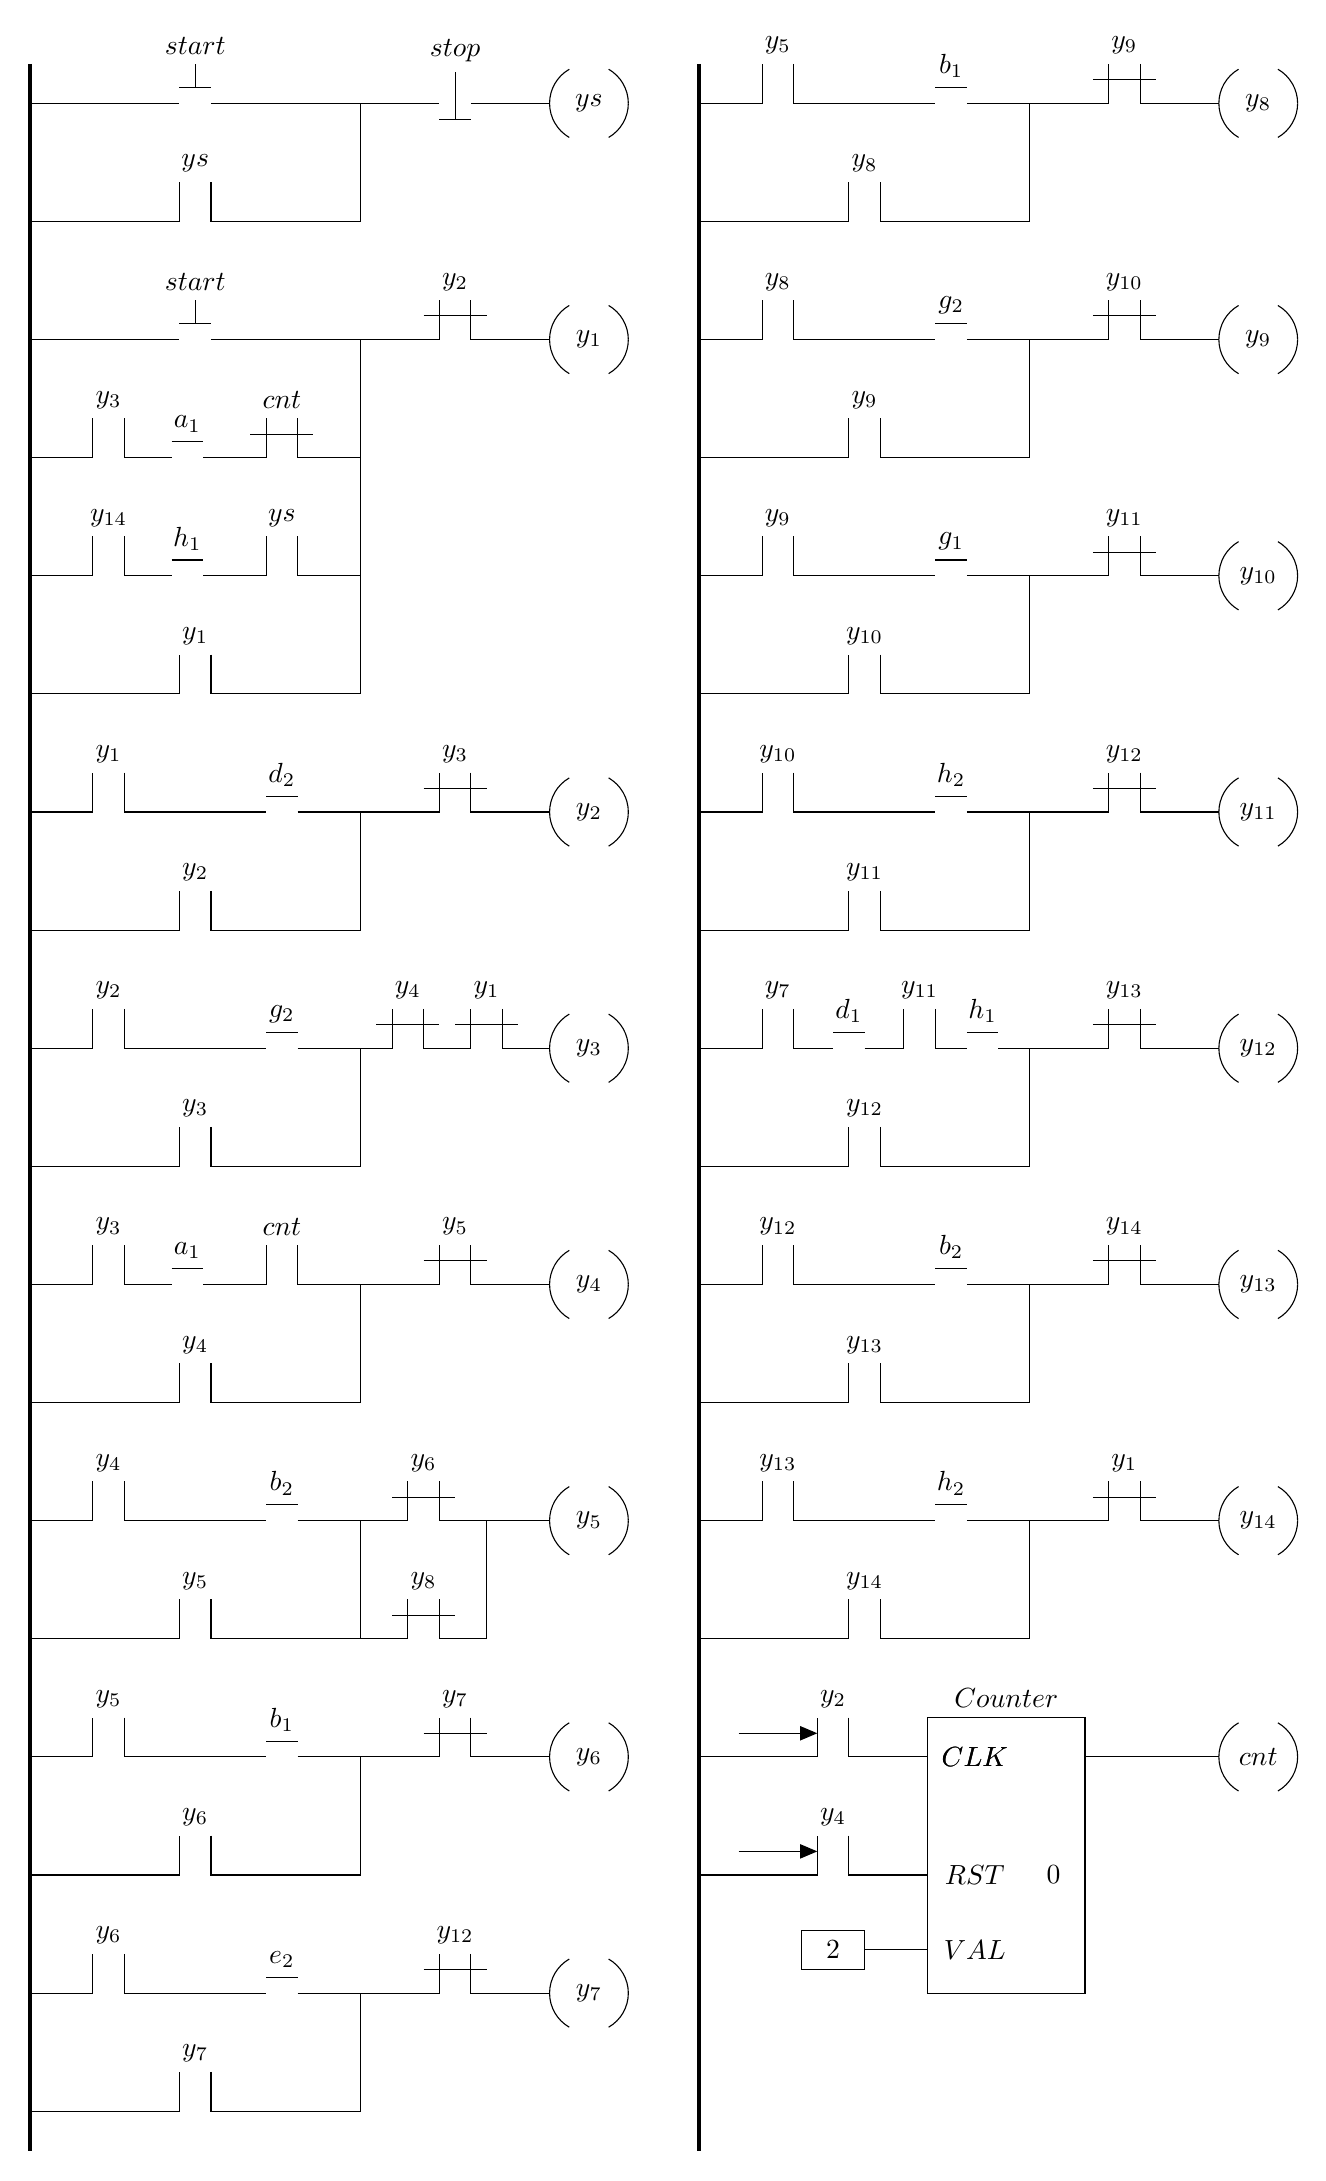
\begin{tikzpicture}[>=triangle 45]
								\draw[ultra thick] (0,0.5) -- (0,-26);
						
								\draw (0,0) -- (1.9,0); \draw (1.9,0.2) -- (2.3, 0.2); \draw (2.1,0.2) -- (2.1, 0.5) node[above]{$start$}; \draw (2.3,0) -- (5.2,0);\draw (5.2,-0.2) -- (5.6,-0.2);  \draw (5.4,-0.2) -- (5.4, 0.4) node[above]{$stop$}; \draw (5.6,0) -- (6.6,0); \draw (6.6,0) arc (180:120:.5);\draw (6.6,0) arc (180:240:.5); \draw (7.6,0) arc (0:60:.5);\draw (7.6,0) arc (0:-60:.5); \draw (7.1,0) node{$ys$}; \draw (0,-1.5) -- (1.9,-1.5) -- (1.9,-1); \draw (2.3,-1) -- (2.3,-1.5) -- (4.2,-1.5) -- (4.2,0); \draw (2.1,-1) node[above]{$ys$};
						
								\draw (0,-3) -- (1.9,-3); \draw (1.9,-2.8) -- (2.3, -2.8); \draw (2.1,-2.8) -- (2.1, -2.5) node[above]{$start$}; \draw (2.3,-3) -- (4.2,-3);
								\draw (0,-4.5) -- (0.8,-4.5) -- (0.8,-4); \draw (1.2,-4) -- (1.2,-4.5) -- (1.8,-4.5); \draw (1,-4) node[above]{$y_3$}; \draw (1.8,-4.3) -- (2.2,-4.3); \draw(2,-4.3) node[above]{$a_1$}; \draw (2.2,-4.5) -- (3,-4.5) -- (3,-4); \draw (3.4,-4) -- (3.4,-4.5) -- (4.2,-4.5); \draw (2.8,-4.2) -- (3.6,-4.2); \draw (3.2,-4) node[above] {$cnt$};
						
								\draw (0,-6) -- (0.8,-6) -- (0.8,-5.5); \draw (1.2,-5.5) -- (1.2,-6)  -- (1.8,-6); \draw (1,-5.5) node[above]{$y_{14}$}; \draw (1.8,-5.8) -- (2.2,-5.8); \draw(2,-5.8) node[above]{$h_{1}$}; \draw (2.2,-6) -- (3,-6) -- (3,-5.5); \draw (3.4,-5.5) -- (3.4,-6) -- (4.2,-6); \draw (3.2,-5.5) node[above] {$ys$};
								\draw (0,-7.5) -- (1.9,-7.5) -- (1.9,-7); \draw (2.3,-7) -- (2.3,-7.5)  -- (4.2,-7.5) -- (4.2,-3); \draw (2.1,-7) node[above]{$y_1$};
						
								\draw (4.2,-3) -- (5.2,-3)-- (5.2,-2.5); \draw (5.6,-2.5) -- (5.6,-3) -- (6.6,-3); \draw (5,-2.7) -- (5.8, -2.7); \draw (5.4,-2.5) node[above]{$y_2$};  \draw (6.6,-3) arc (180:120:.5);\draw (6.6,-3) arc (180:240:.5); \draw (7.6,-3) arc (0:60:.5);\draw (7.6,-3) arc (0:-60:.5); \draw (7.1,-3) node{$y_1$};
						
						
								\draw (0,-9) -- (0.8,-9) -- (0.8,-8.5); \draw (1.2,-8.5) -- (1.2,-9) -- (3,-9); \draw (1,-8.5) node[above]{$y_1$};  \draw (3,-8.8) -- (3.4,-8.8); \draw(3.2,-8.8) node[above]{$d_2$}; \draw (3.4,-9) -- (4.2,-9); \draw (4.2,-9) -- (5.2,-9)-- (5.2,-8.5); \draw (5.6,-8.5) -- (5.6,-9) -- (6.6,-9); \draw (5,-8.7) -- (5.8, -8.7); \draw (5.4,-8.5) node[above]{$y_3$}; \draw (6.6,-9) arc (180:120:.5);\draw (6.6,-9) arc (180:240:.5); \draw (7.6,-9) arc (0:60:.5);\draw (7.6,-9) arc (0:-60:.5); \draw (7.1,-9) node{$y_2$}; \draw (0,-10.5) -- (1.9,-10.5) -- (1.9,-10); \draw (2.3,-10) -- (2.3,-10.5) -- (4.2,-10.5) -- (4.2,-9); \draw (2.1,-10) node[above]{$y_2$};
						
								\draw (0,-12) -- (0.8,-12) -- (0.8,-11.5); \draw (1.2,-11.5) -- (1.2,-12) -- (3,-12); \draw (1,-11.5) node[above]{$y_2$}; \draw (3,-11.8) -- (3.4,-11.8); \draw(3.2,-11.8) node[above]{$g_2$}; \draw (3.4,-12) -- (4.2,-12); 
								\draw (4.2,-12) -- (4.6,-12)-- (4.6,-11.5); \draw (5,-11.5) -- (5,-12) -- (5.6,-12); \draw (4.4,-11.7) -- (5.2, -11.7); \draw (4.8,-11.5) node[above]{$y_4$}; 
								\draw  (5.6,-12)-- (5.6,-11.5); \draw (6,-11.5) -- (6,-12) -- (6.6,-12); \draw (5.4,-11.7) -- (6.2, -11.7); \draw (5.8,-11.5) node[above]{$y_1$}; 
								\draw (6.6,-12) arc (180:120:.5);\draw (6.6,-12) arc (180:240:.5); \draw (7.6,-12) arc (0:60:.5);\draw (7.6,-12) arc (0:-60:.5); \draw (7.1,-12) node{$y_3$}; \draw (0,-13.5) -- (1.9,-13.5) -- (1.9,-13); \draw (2.3,-13) -- (2.3,-13.5) -- (4.2,-13.5) -- (4.2,-12); \draw (2.1,-13) node[above]{$y_3$}; 
						
								\draw (0,-15) -- (0.8,-15) -- (0.8,-14.5); \draw (1.2,-14.5) -- (1.2,-15) -- (1.8,-15); \draw (1,-14.5) node[above]{$y_{3}$};  \draw (1.8,-14.8) -- (2.2,-14.8); \draw(2,-14.8) node[above]{$a_{1}$}; \draw (2.2,-15) -- (3,-15) -- (3,-14.5); \draw (3.4,-14.5) -- (3.4,-15) -- (4.2,-15); \draw (3.2,-14.5) node[above] {$cnt$};
						
								\draw (4.2,-15) -- (5.2,-15)-- (5.2,-14.5); \draw (5.6,-14.5) -- (5.6,-15) -- (6.6,-15); \draw (5,-14.7) -- (5.8, -14.7); \draw (5.4,-14.5) node[above]{$y_5$};\draw (6.6,-15) arc (180:120:.5);\draw (6.6,-15) arc (180:240:.5); \draw (7.6,-15) arc (0:60:.5);\draw (7.6,-15) arc (0:-60:.5); \draw (7.1,-15) node{$y_4$};
						
								\draw (0,-16.5) -- (1.9,-16.5) -- (1.9,-16); \draw (2.3,-16) -- (2.3,-16.5) -- (4.2,-16.5) -- (4.2,-15); \draw (2.1,-16) node[above]{$y_4$}; 
						
						
								\draw (0,-18) -- (0.8,-18) -- (0.8,-17.5); \draw (1.2,-17.5) -- (1.2,-18) -- (3,-18); \draw (1,-17.5) node[above]{$y_4$}; \draw (3,-17.8) -- (3.4,-17.8); \draw(3.2,-17.8) node[above]{$b_2$}; \draw (3.4,-18) -- (4.2,-18); \draw (4.2,-18) -- (4.8,-18)-- (4.8,-17.5); \draw (5.2,-17.5) -- (5.2,-18) -- (6.6,-18); \draw (4.6,-17.7) -- (5.4, -17.7); \draw (5,-17.5) node[above]{$y_6$}; 
								\draw (6.6,-18) arc (180:120:.5);\draw (6.6,-18) arc (180:240:.5); \draw (7.6,-18) arc (0:60:.5);\draw (7.6,-18) arc (0:-60:.5); \draw (7.1,-18) node{$y_5$}; \draw (0,-19.5) -- (1.9,-19.5) -- (1.9,-19); \draw (2.3,-19) -- (2.3,-19.5) -- (4.2,-19.5) -- (4.2,-18); \draw (2.1,-19) node[above]{$y_5$};
						
								\draw (4.2,-19.5) -- (4.8,-19.5)-- (4.8,-19); \draw (5.2,-19) -- (5.2,-19.5) -- (5.8,-19.5) -- (5.8,-18); \draw (4.6,-19.2) -- (5.4, -19.2); \draw (5,-19) node[above]{$y_8$}; 
						
								\draw (0,-21) -- (0.8,-21)-- (0.8,-20.5); \draw (1.2,-20.5) -- (1.2,-21)-- (3,-21); \draw (1,-20.5) node[above]{$y_5$};  \draw (3,-20.8) -- (3.4,-20.8); \draw(3.2,-20.8) node[above]{$b_1$}; \draw (3.4,-21) -- (4.2,-21); \draw (4.2,-21) -- (5.2,-21)-- (5.2,-20.5); \draw (5.6,-20.5) -- (5.6,-21) -- (6.6,-21); \draw (5,-20.7) -- (5.8, -20.7); \draw (5.4,-20.5) node[above]{$y_7$};  \draw (6.6,-21) arc (180:120:.5);\draw (6.6,-21) arc (180:240:.5); \draw (7.6,-21) arc (0:60:.5);\draw (7.6,-21) arc (0:-60:.5); \draw (7.1,-21) node{$y_6$}; \draw (0,-22.5) -- (1.9,-22.5) -- (1.9,-22); \draw (2.3,-22) -- (2.3,-22.5)  -- (4.2,-22.5) -- (4.2,-21); \draw (2.1,-22) node[above]{$y_6$}; 
						
								\draw (0,-24) -- (0.8,-24) -- (0.8,-23.5); \draw (1.2,-23.5) -- (1.2,-24) -- (3,-24); \draw (1,-23.5) node[above]{$y_6$}; \draw (3,-23.8) -- (3.4,-23.8); \draw(3.2,-23.8) node[above]{$e_2$}; \draw (3.4,-24) -- (4.2,-24); \draw (4.2,-24) -- (5.2,-24)-- (5.2,-23.5); \draw (5.6,-23.5) -- (5.6,-24) -- (6.6,-24); \draw (5,-23.7) -- (5.8, -23.7); \draw (5.4,-23.5) node[above]{$y_{12}$}; \draw (6.6,-24) arc (180:120:.5);\draw (6.6,-24) arc (180:240:.5); \draw (7.6,-24) arc (0:60:.5);\draw (7.6,-24) arc (0:-60:.5); \draw (7.1,-24) node{$y_7$}; \draw (0,-25.5) -- (1.9,-25.5) -- (1.9,-25); \draw (2.3,-25) -- (2.3,-25.5)-- (4.2,-25.5) -- (4.2,-24); \draw (2.1,-25) node[above]{$y_7$}; 
						
								\draw[ultra thick] (8.5,0.5) -- (8.5,-26);
						
								\draw (8.5,0) -- (9.3,0) -- (9.3,0.5); \draw (9.7,0.5) -- (9.7,0) -- (11.5,0); \draw (9.5,0.5) node[above]{$y_5$}; \draw (11.5,0.2) -- (11.9,0.2); \draw(11.7,0.2) node[above]{$b_1$}; \draw (11.9,0) -- (12.7,0); \draw (12.7,0) -- (13.7,0)-- (13.7,0.5); \draw (14.1,0.5) -- (14.1,0)-- (15.1,0); \draw (13.5,0.3) -- (14.3, 0.3); \draw (13.9,0.5) node[above]{$y_9$};  \draw (15.1,0) arc (180:120:.5);\draw (15.1,0) arc (180:240:.5); \draw (16.1,0) arc (0:60:.5);\draw (16.1,0) arc (0:-60:.5); \draw (15.6,0) node{$y_8$}; \draw (8.5,-1.5) -- (10.4,-1.5) -- (10.4,-1); \draw (10.8,-1) -- (10.8,-1.5)-- (12.7,-1.5) -- (12.7,0); \draw (10.6,-1) node[above]{$y_8$};
						
								\draw (8.5,-3) -- (9.3,-3) -- (9.3,-2.5); \draw (9.7,-2.5) -- (9.7,-3) -- (11.5,-3); \draw (9.5,-2.5) node[above]{$y_8$};  \draw (11.5,-2.8) -- (11.9,-2.8); \draw(11.7,-2.8) node[above]{$g_2$}; \draw (11.9,-3) -- (12.7,-3); \draw (12.7,-3) -- (13.7,-3)-- (13.7,-2.5); \draw (14.1,-2.5) -- (14.1,-3) -- (15.1,-3); \draw (13.5,-2.7) -- (14.3, -2.7); \draw (13.9,-2.5) node[above]{$y_{10}$};\draw (15.1,-3) arc (180:120:.5);\draw (15.1,-3) arc (180:240:.5); \draw (16.1,-3) arc (0:60:.5);\draw (16.1,-3) arc (0:-60:.5); \draw (15.6,-3) node{$y_9$}; \draw (8.5,-4.5) -- (10.4,-4.5) -- (10.4,-4); \draw (10.8,-4) -- (10.8,-4.5)-- (12.7,-4.5) -- (12.7,-3); \draw (10.6,-4) node[above]{$y_9$};
						
								\draw (8.5,-6) -- (9.3,-6) -- (9.3,-5.5); \draw (9.7,-5.5) -- (9.7,-6) -- (11.5,-6); \draw (9.5,-5.5) node[above]{$y_9$};  \draw (11.5,-5.8) -- (11.9,-5.8); \draw(11.7,-5.8) node[above]{$g_1$}; \draw (11.9,-6) -- (12.7,-6); \draw (12.7,-6) -- (13.7,-6)-- (13.7,-5.5); \draw (14.1,-5.5) -- (14.1,-6) -- (15.1,-6); \draw (13.5,-5.7) -- (14.3, -5.7); \draw (13.9,-5.5) node[above]{$y_{11}$}; \draw (15.1,-6) arc (180:120:.5);\draw (15.1,-6) arc (180:240:.5); \draw (16.1,-6) arc (0:60:.5);\draw (16.1,-6) arc (0:-60:.5); \draw (15.6,-6) node{$y_{10}$}; \draw (8.5,-7.5) -- (10.4,-7.5) -- (10.4,-7); \draw (10.8,-7) -- (10.8,-7.5)-- (12.7,-7.5) -- (12.7,-6); \draw (10.6,-7) node[above]{$y_{10}$};
						
								\draw (8.5,-9) -- (9.3,-9) -- (9.3,-8.5); \draw (9.7,-8.5) -- (9.7,-9)-- (11.5,-9); \draw (9.5,-8.5) node[above]{$y_{10}$}; \draw (11.5,-8.8) -- (11.9,-8.8); \draw(11.7,-8.8) node[above]{$h_2$}; \draw (11.9,-9) -- (12.7,-9); \draw (12.7,-9) -- (13.7,-9)-- (13.7,-8.5); \draw (14.1,-8.5) -- (14.1,-9) -- (15.1,-9); \draw (13.5,-8.7) -- (14.3, -8.7); \draw (13.9,-8.5) node[above]{$y_{12}$}; \draw (15.1,-9) arc (180:120:.5);\draw (15.1,-9) arc (180:240:.5); \draw (16.1,-9) arc (0:60:.5);\draw (16.1,-9) arc (0:-60:.5); \draw (15.6,-9) node{$y_{11}$}; \draw (8.5,-10.5) -- (10.4,-10.5) -- (10.4,-10); \draw (10.8,-10) -- (10.8,-10.5) -- (12.7,-10.5) -- (12.7,-9); \draw (10.6,-10) node[above]{$y_{11}$}; 
						
								\draw (8.5,-12) -- (9.3,-12) -- (9.3,-11.5); \draw (9.7,-11.5) -- (9.7,-12) -- (10.2,-12); \draw (9.5,-11.5) node[above]{$y_7$};  \draw (10.2,-11.8) -- (10.6,-11.8); \draw (10.4,-11.8) node[above] {$d_{1}$}; \draw (10.6,-12) -- (11.1,-12) -- (11.1,-11.5); \draw (11.5,-11.5) -- (11.5,-12) -- (11.9,-12); \draw (11.3,-11.5) node[above]{$y_{11}$};  \draw (11.9,-11.8) --  (12.3,-11.8); \draw (12.1,-11.8) node[above]{$h_{1}$}; \draw (12.3,-12) -- (13.7,-12) -- (13.7,-11.5); \draw (14.1,-11.5) -- (14.1,-12); \draw (13.5,-11.7) -- (14.3, -11.7); \draw (13.9,-11.5) node[above]{$y_{13}$}; \draw (14.1,-12) -- (15.1,-12); \draw (15.1,-12) arc (180:120:.5);\draw (15.1,-12) arc (180:240:.5); \draw (16.1,-12) arc (0:60:.5);\draw (16.1,-12) arc (0:-60:.5); \draw (15.6,-12) node{$y_{12}$}; \draw (8.5,-13.5) -- (10.4,-13.5) -- (10.4,-13); \draw (10.8,-13) -- (10.8,-13.5) -- (12.7,-13.5) -- (12.7,-12); \draw (10.6,-13) node[above]{$y_{12}$};
						
								\draw (8.5,-15) -- (9.3,-15) -- (9.3,-14.5); \draw (9.7,-14.5) -- (9.7,-15) -- (11.5,-15); \draw (9.5,-14.5) node[above]{$y_{12}$};  \draw (11.5,-14.8) -- (11.9,-14.8); \draw(11.7,-14.8) node[above]{$b_2$}; \draw (11.9,-15) -- (12.7,-15); \draw (12.7,-15) -- (13.7,-15)-- (13.7,-14.5); \draw (14.1,-14.5) -- (14.1,-15)-- (15.1,-15); \draw (13.5,-14.7) -- (14.3, -14.7); \draw (13.9,-14.5) node[above]{$y_{14}$}; \draw (15.1,-15) arc (180:120:.5);\draw (15.1,-15) arc (180:240:.5); \draw (16.1,-15) arc (0:60:.5);\draw (16.1,-15) arc (0:-60:.5); \draw (15.6,-15) node{$y_{13}$}; \draw (8.5,-16.5) -- (10.4,-16.5) -- (10.4,-16); \draw (10.8,-16) -- (10.8,-16.5)  -- (12.7,-16.5) -- (12.7,-15); \draw (10.6,-16) node[above]{$y_{13}$};
						
								\draw (8.5,-18) -- (9.3,-18) -- (9.3,-17.5); \draw (9.7,-17.5) -- (9.7,-18) -- (11.5,-18); \draw (9.5,-17.5) node[above]{$y_{13}$};  \draw (11.5,-17.8) -- (11.9,-17.8); \draw(11.7,-17.8) node[above]{$h_2$}; \draw (11.9,-18) -- (12.7,-18); \draw (12.7,-18) -- (13.7,-18)-- (13.7,-17.5); \draw (14.1,-17.5) -- (14.1,-18)-- (15.1,-18); \draw (13.5,-17.7) -- (14.3, -17.7); \draw (13.9,-17.5) node[above]{$y_{1}$};  \draw (15.1,-18) arc (180:120:.5);\draw (15.1,-18) arc (180:240:.5); \draw (16.1,-18) arc (0:60:.5);\draw (16.1,-18) arc (0:-60:.5); \draw (15.6,-18) node{$y_{14}$}; \draw (8.5,-19.5) -- (10.4,-19.5) -- (10.4,-19); \draw (10.8,-19) -- (10.8,-19.5)  -- (12.7,-19.5) -- (12.7,-18); \draw (10.6,-19) node[above]{$y_{14}$}; 
						
								\draw (8.5,-21) -- (10,-21) -- (10,-20.5); \draw (10.4,-20.5) -- (10.4,-21) -- (11.4,-21);  \draw[->] (9,-20.7) -- (10,-20.7); \draw (10.2,-20.5) node[above]{$y_2$}; \draw (12,-21) node {$CLK$}; \draw (11.4,-20.5) rectangle (13.4,-24); \draw (8.5,-22.5) -- (10,-22.5) -- (10,-22); \draw (10.4,-22) -- (10.4,-22.5) -- (11.4,-22.5); \draw[->] (9,-22.2) -- (10,-22.2); \draw (10.2,-22) node[above]{$y_4$}; \draw (12,-22.5) node {$RST$}; \draw (13,-22.5) node {$0$};\draw (9.8,-23.2) rectangle (10.6,-23.7); \draw (10.2,-23.45) node{$2$}; \draw (10.6,-23.45) -- (11.4,-23.45); \draw (12,-23.45) node {$VAL$}; \draw (12,-21) node {$CLK$}; \draw (12.4,-20.5) node[above] {$Counter$}; \draw (13.4,-21) -- (15.1,-21); \draw (15.1,-21) arc (180:120:.5);\draw (15.1,-21) arc (180:240:.5); \draw (16.1,-21) arc (0:60:.5);\draw (16.1,-21) arc (0:-60:.5); \draw (15.6,-21) node{$cnt$};
							\end{tikzpicture}
						\end{center}
					\end{figure}
				
				\item \emph{Bước 4: Viết sơ đồ cấp điện.} Khi viết sơ đồ cấp điện chúng ta không cần quan tâm đến vòng lặp của quá trình, sơ đồ cấp điện được biểu diễn trên \emph{hình \ref{Fig:quatrinh-tuantu-baitap4-sodocapdien}}.
					\begin{figure}[!h]
						\vspace{-.5cm}
						\begin{center}
							\begin{tikzpicture}[>=triangle 45]
								\draw (5,0) node {\small{$Start~A+D+D-G+G-A-A+B+A-B-\left\{\begin{array}{c}D+E+E-D-\\ \\G+G-H+H-\end{array}\right\}E+B+B-H+E-H-$}};								
								\draw[thick] (-2.6,0.5) -- (-2.8,-0.2);
								\draw[thick] (-1,0.5) -- (-1.2,-0.2); \draw (-1.75,0.5) node[above]{$y_1$};
						
								\draw[thick] (0.55,0.5) -- (0.35,-0.2); \draw (-0.25,0.5) node[above]{$y_2$};
						
								\draw[thick] (2.1,0.5) -- (1.9,-0.2); \draw (1.25,0.5) node[above]{$y_3$};
						
								\draw[thick] (3.65,0.5) -- (3.45,-0.2); \draw (2.875,0.5) node[above]{$y_4$};
						
								\draw[thick] (5.15,0.5) -- (5,-0.2); \draw (4.4,0.5) node[above]{$y_5$};
						
								\draw[thick] (5.6,1) -- (5.5,0.3);
								\draw[thick] (7.2,1) -- (7.1,0.3); \draw (6.175,1) node[above]{$y_6$};
						
								\draw[thick] (8.7,1) -- (8.6,0.3); \draw (7.95,1) node[above]{$y_7$};
							
								\draw[thick] (5.6,0) -- (5.45,-.8);
								\draw[thick] (6.4,0) -- (6.25,-.8); \draw (5.8,-.8) node[below]{$y_8$};
						
								\draw[thick] (7.2,0) -- (7.05,-.8); \draw (6.7,-0.8) node[below]{$y_9$};
						
								\draw[thick] (8,0) -- (7.85,-.8); \draw (7.5,-.8) node[below]{$y_{10}$};
						
								\draw[thick] (8.8,0) -- (8.65,-.8); \draw (8.3,-.8) node[below]{$y_{11}$};
						
								\draw[thick] (9.2,0.5) -- (9.05,-0.2);						
								\draw[thick] (10.8,0.5) -- (10.65,-0.2); \draw (10,.5) node[above]{$y_{12}$};
						
								\draw[thick] (12.4,0.5) -- (12.25,-0.2); \draw (11.6,.5) node[above]{$y_{13}$};
						
								\draw[thick] (14,0.5) -- (13.85,-0.2); \draw (13.2,.5) node[above]{$y_{14}$};
								
								\draw(-3.2,-2) node{$A$};
								\draw[thick] (-2.7,-2) -- (-1.2,-2); \draw[thick] (-2.7,-1.8) -- (-2.7,-2.2); \draw[thick] (-1.2,-1.8) -- (-1.2,-2.2);
								
								\draw[thick] (-1.2,-2) -- (0.3,-2); \draw[thick] (0.3,-1.8) -- (0.3,-2.2);
								\draw[thick] (0.3,-2) -- (1.2,-2); \draw[thick] (1.2,-1.8) -- (1.2,-2.2);
								
								\draw[thick] (1.9,-2) -- (3.5,-2); \draw[thick] (1.9,-1.8) -- (1.9,-2.2); \draw[thick] (3.5,-1.8) -- (3.5,-2.2);
								
								
								\draw(-3.2,-3) node{$B$};
								\draw[thick] (2.7,-3) -- (3.5,-3); \draw[thick] (2.7,-2.8) -- (2.7,-3.2); \draw[thick] (3.5,-2.8) -- (3.5,-3.2);
								
								\draw[thick] (3.5,-3) -- (4.2,-3);  \draw[thick] (4.2,-2.8) -- (4.2,-3.2);
								
								\draw[thick] (9.9,-3) -- (10.7,-3); \draw[thick] (9.9,-2.8) -- (9.9,-3.2); \draw[thick] (10.7,-2.8) -- (10.7,-3.2);
								
								
								\draw(-3.2,-4) node{$D$};
								
								\draw[thick] (-1.95,-4) -- (-1.2,-4); \draw[thick] (-1.95,-3.8) -- (-1.95,-4.2); \draw[thick] (-1.2,-3.8) -- (-1.2,-4.2);
								
								\draw[thick] (5.5,-4) -- (7.1,-4);  \draw[thick] (5.5,-3.8) -- (5.5,-4.2); \draw[thick] (7.1,-3.8) -- (7.1,-4.2);
								
								\draw[thick] (7.1,-4) -- (7.9,-4);  \draw[thick] (7.9,-3.8) -- (7.9,-4.2);
			
								
								\draw(-3.2,-5) node{$E$};
								
								\draw[thick] (6.4,-5) -- (7.1,-5);  \draw[thick] (6.4,-4.8) -- (6.4,-5.2); \draw[thick] (7.1,-4.8) -- (7.1,-5.2);
								
								\draw[thick] (9.2,-5) -- (10.7,-5); \draw[thick] (9.2,-4.8) -- (9.2,-5.2); \draw[thick] (10.7,-4.8) -- (10.7,-5.2);
								
								\draw[thick] (10.7,-5) -- (12.3,-5);  \draw[thick] (12.3,-4.8) -- (12.3,-5.2);

								
								\draw(-3.2,-6) node{$G$};
								
								\draw[thick] (-0.4,-6) -- (0.3,-6); \draw[thick] (-0.4,-5.8) -- (-0.4,-6.2); \draw[thick] (0.3,-5.8) -- (0.3,-6.2);
								
								\draw[thick] (5.5,-6) -- (6.4,-6);  \draw[thick] (5.5,-5.8) -- (5.5,-6.2); \draw[thick] (6.4,-5.8) -- (6.4,-6.2);
								
								\draw(-3.2,-7) node{$H$};
								
								\draw[thick] (7.1,-7) -- (7.9,-7);  \draw[thick] (7.1,-6.8) -- (7.1,-7.2); \draw[thick] (7.9,-6.8) -- (7.9,-7.2);
								
								\draw[thick] (11.5,-7) -- (12.3,-7); \draw[thick] (11.5,-6.8) -- (11.5,-7.2); \draw[thick] (12.3,-6.8) -- (12.3,-7.2);
								
								\draw[thick] (12.3,-7) -- (13.1,-7); \draw[thick] (13.1,-6.8) -- (13.1,-7.2);
							\end{tikzpicture}
						\end{center}					
					\end{figure}
					
					\begin{figure}[!h]
						\begin{center}
							\begin{tikzpicture}[>=triangle 45]
								\draw[ultra thick] (0,0.5) -- (0,-14);
								\draw (0,0) -- (1.9,0) -- (1.9,0.5); \draw (2.2,0.5) node[above]{$y_1$}; \draw (2.3,0.5) -- (2.3,0) -- (4.2,0) -- (5.6,0);
								\draw (0,-1.5) -- (1.9,-1.5) -- (1.9,-1); \draw (2.2,-1) node[above]{$y_2$}; \draw (2.3,-1) -- (2.3,-1.5) -- (4.2,-1.5);
								\draw (0,-3) -- (0.8,-3) -- (0.8,-2.5); \draw (1.2,-2.5) -- (1.2,-3) -- (3,-3); \draw (1,-2.5) node[above]{$y_3$}; \draw (3,-3.2) -- (3.4,-3.2); \draw(3.2,-2.8) node[above]{$g_1$}; \draw (3.4,-3) -- (4.2,-3);
								\draw (0,-4.5) -- (1.9,-4.5) -- (1.9,-4); \draw (2.2,-4) node[above]{$y_4$}; \draw (2.3,-4) -- (2.3,-4.5) -- (4.2,-4.5) -- (4.2,0);
								\draw (5.6,0) arc (180:120:.5);\draw (5.6,0) arc (180:240:.5); \draw (6.6,0) arc (0:60:.5);\draw (6.6,0) arc (0:-60:.5); \draw (6.1,0) node{$A$};
								
								
								\draw (0,-6) -- (0.8,-6) -- (0.8,-5.5); \draw (1.2,-5.5) -- (1.2,-6) -- (3,-6); \draw (1,-5.5) node[above]{$y_4$}; \draw (3,-5.8) -- (3.4,-5.8); \draw(3.2,-5.8) node[above]{$a_2$}; \draw (3.4,-6) -- (4.2,-6) -- (5.6,-6);
								\draw (0,-7.5) -- (0.8,-7.5) -- (0.8,-7); \draw (1.2,-7) -- (1.2,-7.5) -- (3,-7.5); \draw (1,-7) node[above]{$y_5$}; \draw (3,-7.7) -- (3.4,-7.7); \draw(3.2,-7.3) node[above]{$a_1$}; \draw (3.4,-7.5) -- (4.2,-7.5);
								\draw (0,-9) -- (0.8,-9) -- (0.8,-8.5); \draw (1.2,-8.5) -- (1.2,-9) -- (3,-9); \draw (1,-8.5) node[above]{$y_{12}$}; \draw (3,-8.8) -- (3.4,-8.8); \draw(3.2,-8.8) node[above]{$e_2$}; \draw (3.4,-9) -- (4.2,-9) -- (4.2,-6);
								\draw (5.6,-6) arc (180:120:.5);\draw (5.6,-6) arc (180:240:.5); \draw (6.6,-6) arc (0:60:.5);\draw (6.6,-6) arc (0:-60:.5); \draw (6.1,-6) node{$B$};
								
								
								\draw (0,-10.5) -- (0.8,-10.5) -- (0.8,-10); \draw (1.2,-10) -- (1.2,-10.5) -- (3,-10.5); \draw (1,-10) node[above]{$y_{1}$}; \draw (3,-10.3) -- (3.4,-10.3); \draw(3.2,-10.3) node[above]{$a_2$}; \draw (3.4,-10.5) -- (4.2,-10.5) -- (5.6,-10.5);
								\draw (0,-12) -- (1.9,-12) -- (1.9,-11.5); \draw (2.2,-11.5) node[above]{$y_6$}; \draw (2.3,-11.5) -- (2.3,-12) -- (4.2,-12);
								\draw (0,-13.5) -- (0.8,-13.5) -- (0.8,-13); \draw (1.2,-13) -- (1.2,-13.5) -- (3,-13.5); \draw (1,-13) node[above]{$y_{7}$}; \draw (3,-13.7) -- (3.4,-13.7); \draw(3.2,-13.3) node[above]{$e_1$}; \draw (3.4,-13.5) -- (4.2,-13.5) -- (4.2,-10.5);
								\draw (5.6,-10.5) arc (180:120:.5);\draw (5.6,-10.5) arc (180:240:.5); \draw (6.6,-10.5) arc (0:60:.5);\draw (6.6,-10.5) arc (0:-60:.5); \draw (6.1,-10.5) node{$D$};
								
								\draw[ultra thick] (7.5,0.5) -- (7.5,-14);
								\draw (7.5,0) -- (8.3,0) -- (8.3,0.5); \draw (8.7,0.5) -- (8.7,0) -- (10.5,0); \draw (8.5,0.5) node[above]{$y_{6}$}; \draw (10.5,0.2) -- (10.9,0.2); \draw(10.7,0.2) node[above]{$d_2$}; \draw (10.9,0) -- (11.7,0) -- (13.1,0);
								\draw (7.5,-1.5) -- (9.4,-1.5) -- (9.4,-1); \draw (9.7,-1) node[above]{$y_{12}$}; \draw (9.8,-1) -- (9.8,-1.5) -- (11.7,-1.5);
								\draw (7.5,-3) -- (9.4,-3) -- (9.4,-2.5); \draw (9.7,-2.5) node[above]{$y_{13}$}; \draw (9.8,-2.5) -- (9.8,-3) -- (11.7,-3) -- (11.7,0);
								\draw (13.1,0) arc (180:120:.5);\draw (13.1,0) arc (180:240:.5); \draw (14.1,0) arc (0:60:.5);\draw (14.1,0) arc (0:-60:.5); \draw (13.6,0) node{$E$};
								
								\draw (7.5,-4.5) -- (8.3,-4.5) -- (8.3,-4); \draw (8.7,-4) -- (8.7,-4.5) -- (10.5,-4.5); \draw (8.5,-4) node[above]{$y_{2}$}; \draw (10.5,-4.3) -- (10.9,-4.3); \draw(10.7,-4.3) node[above]{$d_1$}; \draw (10.9,-4.5) -- (11.7,-4.5) -- (13.1,-4.5);
								\draw (7.5,-6) -- (9.4,-6) -- (9.4,-5.5); \draw (9.7,-5.5) node[above]{$y_{8}$}; \draw (9.8,-5.5) -- (9.8,-6) -- (11.7,-6) -- (11.7,-4.5);
								\draw (13.1,-4.5) arc (180:120:.5);\draw (13.1,-4.5) arc (180:240:.5); \draw (14.1,-4.5) arc (0:60:.5);\draw (14.1,-4.5) arc (0:-60:.5); \draw (13.6,-4.5) node{$G$};
								
								\draw (7.5,-7.5) -- (9.4,-7.5) -- (9.4,-7); \draw (9.7,-7) node[above]{$y_{10}$}; \draw (9.8,-7) -- (9.8,-7.5) -- (11.7,-7.5) -- (13.1,-7.5);
								\draw (7.5,-9) -- (8.3,-9) -- (8.3,-8.5); \draw (8.7,-8.5) -- (8.7,-9) -- (10.5,-9); \draw (8.5,-8.5) node[above]{$y_{13}$}; \draw (10.5,-8.8) -- (10.9,-8.8); \draw(10.7,-8.8) node[above]{$b_1$}; \draw (10.9,-9) -- (11.7,-9);
								
								\draw (7.5,-10.5) -- (8.3,-10.5) -- (8.3,-10); \draw (8.7,-10) -- (8.7,-10.5) -- (10.5,-10.5); \draw (8.5,-10) node[above]{$y_{14}$}; \draw (10.5,-10.7) -- (10.9,-10.7); \draw(10.7,-10.3) node[above]{$e_1$}; \draw (10.9,-10.5) -- (11.7,-10.5) -- (11.7,-7.5);
								
								\draw (13.1,-7.5) arc (180:120:.5);\draw (13.1,-7.5) arc (180:240:.5); \draw (14.1,-7.5) arc (0:60:.5);\draw (14.1,-7.5) arc (0:-60:.5); \draw (13.6,-7.5) node{$H$};
							\end{tikzpicture}
						\end{center}
						\caption{Sơ đồ cấp điện cho quá trình} \label{Fig:quatrinh-tuantu-baitap4-sodocapdien}
					\end{figure}					
			\end{itemize}
\end{document}